% Figures/pi-vs-vi.tex
% Policy iteration against value function iteration on a random finite Markov
% decision problem, illustrating Theorem \ref{thm:policy-iteration}(ii) of
% Chapter \ref{ch:dynamic}: from the same starting function W_0 the policy
% iterates dominate the value iterates at every step.
% 40 states, 8 actions, beta = 0.95, rewards uniform on [0,1], transition rows
% drawn as normalised cubes of uniforms so that the chains are not close to
% uniform.  Both algorithms start from the value of the same stationary policy.
% The coordinates were produced in MATLAB R2025b; the reference limit V was
% computed by 20000 value-iteration sweeps.  Columns: sweep index m,
% ||W_m - V||_inf under policy iteration, the same under value iteration, and
% the geometric envelope beta^m ||W_0 - V||_inf.
% Generator: Figures/matlab/pi_vs_vi_data.m, which writes pi-vs-vi.dat; the
% tables below are that file verbatim.  Rerun it to regenerate them.
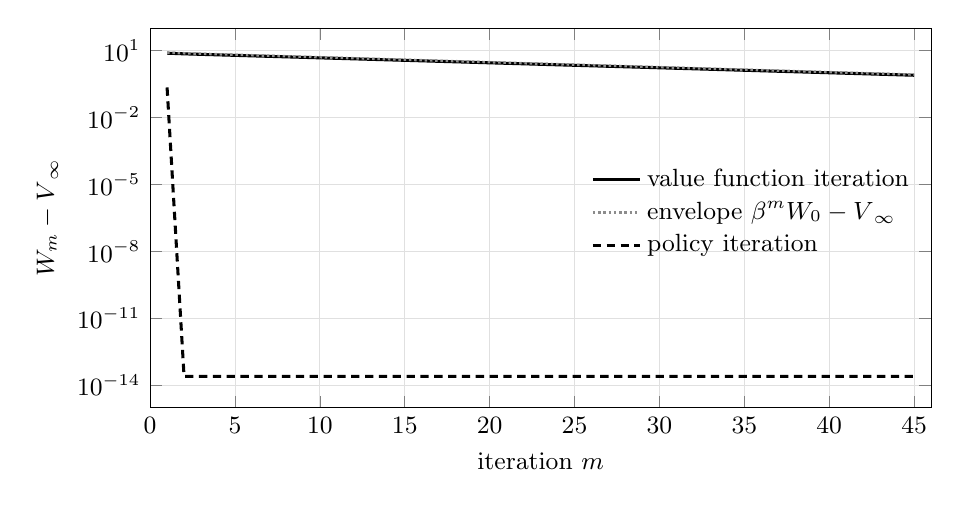
\begin{tikzpicture}
	\begin{semilogyaxis}[
			width=11.5cm, height=6.4cm,
			xlabel={iteration $m$},
			ylabel={$\norm{W_m-V}_\infty$},
			xmin=0, xmax=46,
			ymin=1e-15, ymax=1e2,
			ytick={1e-14,1e-11,1e-8,1e-5,1e-2,1e1},
			tick label style={font=\small},
			label style={font=\small},
			legend cell align=left,
			legend style={draw=none, fill=none, font=\small,
					at={(0.99,0.66)}, anchor=north east},
			grid=major,
			grid style={line width=0.3pt, draw=black!12},
		]
		\addplot[line width=1.1pt, mark=none] table[x index=0, y index=2] {
				1 2.2179551349e-01 7.6079193299e+00 7.9675738255e+00
				2 2.4868995752e-14 7.1224199582e+00 7.5691951342e+00
				3 2.4868995752e-14 6.7465506007e+00 7.1907353775e+00
				4 2.4868995752e-14 6.4062691500e+00 6.8311986087e+00
				5 2.4868995752e-14 6.0853967868e+00 6.4896386782e+00
				6 2.4868995752e-14 5.7809940599e+00 6.1651567443e+00
				7 2.4868995752e-14 5.4919241232e+00 5.8568989071e+00
				8 2.4868995752e-14 5.2173248913e+00 5.5640539617e+00
				9 2.4868995752e-14 4.9564580540e+00 5.2858512637e+00
				10 2.4868995752e-14 4.7086350764e+00 5.0215587005e+00
				11 2.4868995752e-14 4.4732033037e+00 4.7704807654e+00
				12 2.4868995752e-14 4.2495431353e+00 4.5319567272e+00
				13 2.4868995752e-14 4.0370659781e+00 4.3053588908e+00
				14 2.4868995752e-14 3.8352126792e+00 4.0900909463e+00
				15 2.4868995752e-14 3.6434520452e+00 3.8855863990e+00
				16 2.4868995752e-14 3.4612794429e+00 3.6913070790e+00
				17 2.4868995752e-14 3.2882154708e+00 3.5067417251e+00
				18 2.4868995752e-14 3.1238046972e+00 3.3314046388e+00
				19 2.4868995752e-14 2.9676144624e+00 3.1648344069e+00
				20 2.4868995752e-14 2.8192337393e+00 3.0065926865e+00
				21 2.4868995752e-14 2.6782720523e+00 2.8562630522e+00
				22 2.4868995752e-14 2.5443584497e+00 2.7134498996e+00
				23 2.4868995752e-14 2.4171405272e+00 2.5777774046e+00
				24 2.4868995752e-14 2.2962835008e+00 2.4488885344e+00
				25 2.4868995752e-14 2.1814693258e+00 2.3264441077e+00
				26 2.4868995752e-14 2.0723958595e+00 2.2101219023e+00
				27 2.4868995752e-14 1.9687760665e+00 2.0996158072e+00
				28 2.4868995752e-14 1.8703372632e+00 1.9946350168e+00
				29 2.4868995752e-14 1.7768204000e+00 1.8949032660e+00
				30 2.4868995752e-14 1.6879793800e+00 1.8001581027e+00
				31 2.4868995752e-14 1.6035804110e+00 1.7101501975e+00
				32 2.4868995752e-14 1.5234013905e+00 1.6246426877e+00
				33 2.4868995752e-14 1.4472313210e+00 1.5434105533e+00
				34 2.4868995752e-14 1.3748697549e+00 1.4662400256e+00
				35 2.4868995752e-14 1.3061262672e+00 1.3929280243e+00
				36 2.4868995752e-14 1.2408199538e+00 1.3232816231e+00
				37 2.4868995752e-14 1.1787789561e+00 1.2571175420e+00
				38 2.4868995752e-14 1.1198400083e+00 1.1942616649e+00
				39 2.4868995752e-14 1.0638480079e+00 1.1345485816e+00
				40 2.4868995752e-14 1.0106556075e+00 1.0778211525e+00
				41 2.4868995752e-14 9.6012282713e-01 1.0239300949e+00
				42 2.4868995752e-14 9.1211668577e-01 9.7273359016e-01
				43 2.4868995752e-14 8.6651085148e-01 9.2409691066e-01
				44 2.4868995752e-14 8.2318530891e-01 8.7789206512e-01
				45 2.4868995752e-14 7.8202604346e-01 8.3399746187e-01
			};
		\addlegendentry{value function iteration}
		\addplot[line width=0.9pt, mark=none, black!45, densely dotted] table[x index=0, y index=3] {
				1 2.2179551349e-01 7.6079193299e+00 7.9675738255e+00
				2 2.4868995752e-14 7.1224199582e+00 7.5691951342e+00
				3 2.4868995752e-14 6.7465506007e+00 7.1907353775e+00
				4 2.4868995752e-14 6.4062691500e+00 6.8311986087e+00
				5 2.4868995752e-14 6.0853967868e+00 6.4896386782e+00
				6 2.4868995752e-14 5.7809940599e+00 6.1651567443e+00
				7 2.4868995752e-14 5.4919241232e+00 5.8568989071e+00
				8 2.4868995752e-14 5.2173248913e+00 5.5640539617e+00
				9 2.4868995752e-14 4.9564580540e+00 5.2858512637e+00
				10 2.4868995752e-14 4.7086350764e+00 5.0215587005e+00
				11 2.4868995752e-14 4.4732033037e+00 4.7704807654e+00
				12 2.4868995752e-14 4.2495431353e+00 4.5319567272e+00
				13 2.4868995752e-14 4.0370659781e+00 4.3053588908e+00
				14 2.4868995752e-14 3.8352126792e+00 4.0900909463e+00
				15 2.4868995752e-14 3.6434520452e+00 3.8855863990e+00
				16 2.4868995752e-14 3.4612794429e+00 3.6913070790e+00
				17 2.4868995752e-14 3.2882154708e+00 3.5067417251e+00
				18 2.4868995752e-14 3.1238046972e+00 3.3314046388e+00
				19 2.4868995752e-14 2.9676144624e+00 3.1648344069e+00
				20 2.4868995752e-14 2.8192337393e+00 3.0065926865e+00
				21 2.4868995752e-14 2.6782720523e+00 2.8562630522e+00
				22 2.4868995752e-14 2.5443584497e+00 2.7134498996e+00
				23 2.4868995752e-14 2.4171405272e+00 2.5777774046e+00
				24 2.4868995752e-14 2.2962835008e+00 2.4488885344e+00
				25 2.4868995752e-14 2.1814693258e+00 2.3264441077e+00
				26 2.4868995752e-14 2.0723958595e+00 2.2101219023e+00
				27 2.4868995752e-14 1.9687760665e+00 2.0996158072e+00
				28 2.4868995752e-14 1.8703372632e+00 1.9946350168e+00
				29 2.4868995752e-14 1.7768204000e+00 1.8949032660e+00
				30 2.4868995752e-14 1.6879793800e+00 1.8001581027e+00
				31 2.4868995752e-14 1.6035804110e+00 1.7101501975e+00
				32 2.4868995752e-14 1.5234013905e+00 1.6246426877e+00
				33 2.4868995752e-14 1.4472313210e+00 1.5434105533e+00
				34 2.4868995752e-14 1.3748697549e+00 1.4662400256e+00
				35 2.4868995752e-14 1.3061262672e+00 1.3929280243e+00
				36 2.4868995752e-14 1.2408199538e+00 1.3232816231e+00
				37 2.4868995752e-14 1.1787789561e+00 1.2571175420e+00
				38 2.4868995752e-14 1.1198400083e+00 1.1942616649e+00
				39 2.4868995752e-14 1.0638480079e+00 1.1345485816e+00
				40 2.4868995752e-14 1.0106556075e+00 1.0778211525e+00
				41 2.4868995752e-14 9.6012282713e-01 1.0239300949e+00
				42 2.4868995752e-14 9.1211668577e-01 9.7273359016e-01
				43 2.4868995752e-14 8.6651085148e-01 9.2409691066e-01
				44 2.4868995752e-14 8.2318530891e-01 8.7789206512e-01
				45 2.4868995752e-14 7.8202604346e-01 8.3399746187e-01
			};
		\addlegendentry{envelope $\beta^{m}\norm{W_0-V}_\infty$}
		\addplot[line width=1.1pt, mark=none, densely dashed] table[x index=0, y index=1] {
				1 2.2179551349e-01 7.6079193299e+00 7.9675738255e+00
				2 2.4868995752e-14 7.1224199582e+00 7.5691951342e+00
				3 2.4868995752e-14 6.7465506007e+00 7.1907353775e+00
				4 2.4868995752e-14 6.4062691500e+00 6.8311986087e+00
				5 2.4868995752e-14 6.0853967868e+00 6.4896386782e+00
				6 2.4868995752e-14 5.7809940599e+00 6.1651567443e+00
				7 2.4868995752e-14 5.4919241232e+00 5.8568989071e+00
				8 2.4868995752e-14 5.2173248913e+00 5.5640539617e+00
				9 2.4868995752e-14 4.9564580540e+00 5.2858512637e+00
				10 2.4868995752e-14 4.7086350764e+00 5.0215587005e+00
				11 2.4868995752e-14 4.4732033037e+00 4.7704807654e+00
				12 2.4868995752e-14 4.2495431353e+00 4.5319567272e+00
				13 2.4868995752e-14 4.0370659781e+00 4.3053588908e+00
				14 2.4868995752e-14 3.8352126792e+00 4.0900909463e+00
				15 2.4868995752e-14 3.6434520452e+00 3.8855863990e+00
				16 2.4868995752e-14 3.4612794429e+00 3.6913070790e+00
				17 2.4868995752e-14 3.2882154708e+00 3.5067417251e+00
				18 2.4868995752e-14 3.1238046972e+00 3.3314046388e+00
				19 2.4868995752e-14 2.9676144624e+00 3.1648344069e+00
				20 2.4868995752e-14 2.8192337393e+00 3.0065926865e+00
				21 2.4868995752e-14 2.6782720523e+00 2.8562630522e+00
				22 2.4868995752e-14 2.5443584497e+00 2.7134498996e+00
				23 2.4868995752e-14 2.4171405272e+00 2.5777774046e+00
				24 2.4868995752e-14 2.2962835008e+00 2.4488885344e+00
				25 2.4868995752e-14 2.1814693258e+00 2.3264441077e+00
				26 2.4868995752e-14 2.0723958595e+00 2.2101219023e+00
				27 2.4868995752e-14 1.9687760665e+00 2.0996158072e+00
				28 2.4868995752e-14 1.8703372632e+00 1.9946350168e+00
				29 2.4868995752e-14 1.7768204000e+00 1.8949032660e+00
				30 2.4868995752e-14 1.6879793800e+00 1.8001581027e+00
				31 2.4868995752e-14 1.6035804110e+00 1.7101501975e+00
				32 2.4868995752e-14 1.5234013905e+00 1.6246426877e+00
				33 2.4868995752e-14 1.4472313210e+00 1.5434105533e+00
				34 2.4868995752e-14 1.3748697549e+00 1.4662400256e+00
				35 2.4868995752e-14 1.3061262672e+00 1.3929280243e+00
				36 2.4868995752e-14 1.2408199538e+00 1.3232816231e+00
				37 2.4868995752e-14 1.1787789561e+00 1.2571175420e+00
				38 2.4868995752e-14 1.1198400083e+00 1.1942616649e+00
				39 2.4868995752e-14 1.0638480079e+00 1.1345485816e+00
				40 2.4868995752e-14 1.0106556075e+00 1.0778211525e+00
				41 2.4868995752e-14 9.6012282713e-01 1.0239300949e+00
				42 2.4868995752e-14 9.1211668577e-01 9.7273359016e-01
				43 2.4868995752e-14 8.6651085148e-01 9.2409691066e-01
				44 2.4868995752e-14 8.2318530891e-01 8.7789206512e-01
				45 2.4868995752e-14 7.8202604346e-01 8.3399746187e-01
			};
		\addlegendentry{policy iteration}
	\end{semilogyaxis}
\end{tikzpicture}
